\section{Problema en medicina}
Queremos poder obtener una imagen de un plano interior del cuerpo humano sin requerir intervención quirúrgica. Se puede lanzar un rayo $X$ en dirección de la recta $L$ a una intensidad inicial $I_0$, y medir su intensidad final $I_1$ al salir del cuerpo. 

Este cambio de intensidad es dependiente de la atenuación del rayo en cada punto del cuerpo. Entonces, el objetivo es utilizar estas mediciones de cambios de intensidad para calcular la atenuación en cada punto del cuerpo, lo cual se utiliza como la imagen que queremos.

\section{Modelamiento matemático}

El modelo tiene los siguientes elementos:
\begin{itemize}
    \item El cuerpo humano es un compacto $\Omega\subseteq \R^2$
    \item La atenuación en un plano es $\rho:\R^2\to\R$ con soporte en $\Omega$, con condiciones de regularidad por determinar
    \item Un rayo X es $L$ una recta en $\R^2$. Sea $\mathcal{L}$ el conjunto de estas rectas.
\end{itemize}

Definimos entonces la transformada de Radon $R[\rho]:\mathcal{L}\to\R$ como tal:

\[
R[\rho](L) := \int_L \rho(x)\,|dx|
\]

Más concretamente, podemos parametrizar $L$ según:

\[
L_{t, \theta} = \{x\in\R^2: \langle x, n_\theta\rangle = t\}
\]

Donde $n_\theta = (\cos(\theta), \sin(\theta))$. Esto nos da permite ver la tranformada como $R: L^1(\R)\to L^1(S^1\times \R)$, con la siguiente expresión:


\[
R[\rho](t, \theta) = \int \rho(x)\delta(\langle x, n_\theta\rangle - t)\, dx
\]


De acá podemos definir dos problemas \citep{kirsch_2022}:
\begin{itemize}
    \item Problema directo: Dado $\rho$, calcular $R[\rho]$
    \item Problema inverso: Dado $R[\rho]$, calcular $\rho$
\end{itemize}

Este problema está motivado por la siguiente relación, que vé al cambio de intensidad de un rayo en la recta $L$ como la integral de la atenuación:

\[
\ln(\frac{I_1}{I_0}) = R[\rho](L)
\]

Esto significa que en el problema en medicina, podemos medir $R[\rho]$ en cualquier recta $L$, y obtener la imagen es calcular $\rho(\Omega)$, por lo cual se planteó como el problema inverso.

\section{Desafios matemáticos}
Al resolver problemas inversos, existen tres problemas clásicos a discutir:
\subsection{Inyectividad}
Queremos demostrar que si $R[\rho_1] = R[\rho_2]$ casi en todas partes, entonces se cumple que $\rho_1 = \rho_2$ casi en todas partes.

Primero, notamos que la forma en que escribimos la transformada de Radon nos da la siguiente relación con la transformada de Fourier:

\[
\int R[\rho](t, \theta)e^{-i\omega t} \, dt = \hat{\rho}(\omega n_\theta)
\]

No solamente permite demostrar inyectividad, sino que podemos obtener una fórmula de inversión explícita \citep{candes_inverse}:

\[
\rho(x) = \frac{1}{2\pi}\int_0^\pi (R[\rho](\cdot, \theta)*h)(\langle x, n_\theta\rangle)\, d\theta
\]

Donde $h$ es tal que $\hat{h} = |\omega|$. 

\subsection{Estabilidad}
Si nos mantenemos en la topología $L^1$, no tenemos estabilidad. De hecho, existe un resultado desastrozo \citep{herman_natterer_1981}: Existe una secuencia $(\rho_n)\subseteq L^1\cap C^\infty$, todas radiales a soporte en la bola unitaria tales que:

\begin{itemize}
    \item $\rho_n$ es acotada en $L^1$
    \item $R\rho_n\to 0$ tanto uniformemente como en sentido $L^1$
    \item $\rho_n$ no converge en ningún punto, ni siquiera converge débilmente
\end{itemize}

Un resultado que sí podemos notar es que $R^{-1}$ es continuo cuando se vé como operador desde $W_{\infty, 0}^1$ a $L_0^\infty$ (ahora usando la información de las derivadas además del soporte compacto). 

Existen otros resultados que extienden la transformada de Radon para poder definir una convergencia de $R^{-1}$ es una topología más débil, pero estos no se cubrirán en esta tarea.

\subsection{Reconstrucción}
La fórmula de inversión propuesta puede ser utilizada como algoritmo práctico de reconstrucción, con la mayor desventaja siendo el problema de inestabilidad antes mostrado. 

Dado que encontrar una transformada de Radon no es un problema difícil, otra manera de reconstrucción es resolver el problema de optimización \citep{candes_opti}:

\[
\min_{\rho}\Vert R[\rho] - \tilde{R}\Vert^2
\]

Con $\tilde{R}$ la transformada medida. El problema de esta forma sigue siendo inestable, así que es posible considerar además estrategias de regularización para mejorar el desempeño contra el ruido. Por ejemplo, podemos resolver el siguiente problema, parametrizado por $\lambda>0$ regularizador:

\[
\min_{\rho}\Vert R[\rho] - \tilde{R}\Vert^2 + \lambda \Vert \rho\Vert^2
\]

\section{Desafios ingenieriles}
Existen varios desafíos de realizar una tomografía. En particular:
\begin{itemize}
    \item Las imágenes deben ser de alta resolución para ser de mayor utilidad. Esto aumenta el costo de cualquier algoritmo
    \item Los rayos X tienen efectos dañinos en el paciente si la dosis es demasiado alta. La reconstrucción debe requerir pocos rayos para poder usarse factiblemente. En particular, la fórmula de inversión no es viable sin discretizar la integral en muy pocos ángulos. \citep{herman_2012}
    \item Para cada plano que queramos representar, se requiere lanzar rayos en una variedad de ángulos, tales que estos puedan dar la información necesaria en la reconstrucción.
\end{itemize}

\section{Simulaciones}
Incluyo simulaciones en Python de una reconstrucción con la siguiente metodología:
\begin{itemize}
    \item Generar una imagen de $16\times 16$ pixeles a través de ruido de Perlin.
    \item Calcular la transformada de Radon con el módulo \textit{scikit-image} \citep{scikit-image}
    \item Intentar recuperar la imagen inicual resolviendo el problema de optimización antes mostrado (sin regularización)
\end{itemize}
\begin{figure}
    \centering
    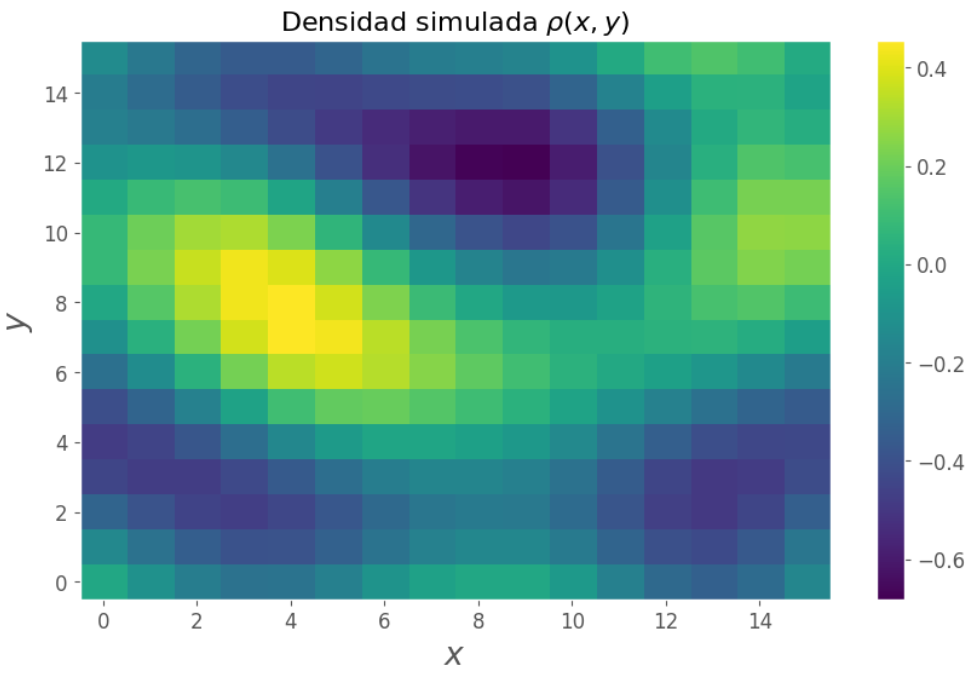
\includegraphics[scale=0.4]{img/simulada.png}
    \caption{Imagen simulada con ruido de Perlin, a reconstruir}
    \label{fig:simulada}
\end{figure}
\begin{figure}
    \centering
    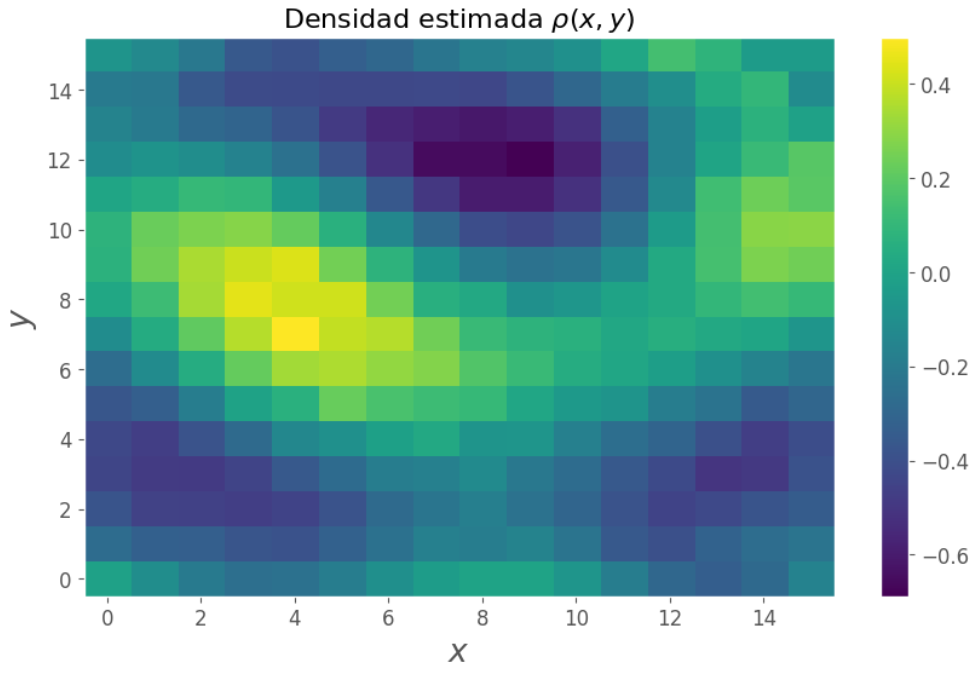
\includegraphics[scale=0.4]{img/estimada.png}
    \caption{Imagen reconstruida a partir de trasnformaciones de Radon}
    \label{fig:estimada}
\end{figure}
Se llegó a una solución en 20 segundos. El error cuadrático medio de las transformadas (el valor que se optimizó) es de $10^{-7}$, mientras que el error de las densidades era de $10^{-4}$.

El repositorio con las simulaciones, y con este informe, se encuentra en \href{https://github.com/johnny-godoy/tomografia-computarizada}{https://github.com/johnny-godoy/tomografia-computarizada}
\bibliography{library.bib}
 